\chapter{范畴论回顾, 方便的空间范畴}
\begin{introduction}
    \item \textbf{范畴论} 是一门数学分支, 最开始由 MacLane 引入以解释自然变换的``自然性''.请读者回忆有限维向量空间 $V$ 与其双重对偶 $(V^{\lor})^{\lor}$ 的自然同构 $\ev_V : V \simeq (V^{\lor})^{\lor}$, 在线性代数中, 我们称该同构是``自然的'', 或 ``典范的'', 以 $\ev_V$ 为例, 一般而言, 可以如下来理解自然性
    
\begin{enumerate}
    \item 它不依赖于基的选取, 事实上, 可以直接写下它的公式 $\ev_V(v) = \left<-,v\right>\colon V^{\lor} \to F$, 这并不需要任意诸如有序基的辅助信息.
    \item 它与线性映射的结构是兼容的, 即
    \[\begin{tikzcd}
	V & W \\
	{V^{\lor \lor}} & {W^{\lor \lor}}
	\arrow["T", from=1-1, to=1-2]
	\arrow["{\ev_V}"', from=1-1, to=2-1]
	\arrow["{\ev_W}", from=1-2, to=2-2]
	\arrow["{T^{\lor \lor}}"', from=2-1, to=2-2]
    \end{tikzcd}\]
\end{enumerate}

\item 范畴论的原理是将不同数学分支的数学理论抽象出来, 只保留两种信息: 数学对象, 以及其间态射(我们所关心的箭头, 或者说是相容的箭头, 例如在我们关心拓扑空间时, 所考虑的箭头即为连续映射, 在关心概形时, 所考虑的箭头往往为概形间的态射). 由此我们可以解释自然或者典范.\\
在考虑从结构 $A$ 中得到结构 $B$ 的信息时(或者说从范畴 $\cal{C}$ 中得到范畴 $\cal{D}$ 的信息, 比方说你考虑带点拓扑空间 $(E,e)$ 的基本群 $\pi_1((E,e))$ 时), 我们就需要用到函子的概念, 上述例子给出了一个函子 $\cate{Top}_{\star} \to \cate{Grp}$(例~\ref{例:范畴}), 更为经典的使用函子的例子是 Brouwer 不动点的证明, 可见定理~\ref{定理:Brouwer}.\\
当然, 函子可能具有一些诸如伴随, 保(余)极限, 可表等性质具体内容我们将在后文进行讨论.\\

\item 在一切开始之前, 我们还需要进行一个观察:
在讨论群的时候, 我们经常认为同构的群是一致的; 在讨论拓扑空间的时候, 我们经常认为同胚的拓扑空间就是一致的.
所以同构/同胚是一种在对应结构中所适用的等号(在对应的代数结构中它往往比严格相等更加有用).因此在范畴论中, 我们自然而然的提出一个朴素观点: \textbf{以同构代替严格等式}.\footnote{当然, 在类型论中, 直接在类型里提出相等类型的概念, 具体分为赋值相等和命题相等, 在此不做过多探讨, 感兴趣的读者请参看类型论相关资料.}

\item 考虑到讨论班参加成员均为初学者, 本文将不会过多讨论 Grothendieck 宇宙的内容, 本文选定一个 Grothendieck 宇宙 $\mathcal{U}$ 若无额外说明, 我们统一认定为小范畴, 即 $\Obj$ 与 $\Mor$ 均为 $\cal{U}$-小集合(即落在 $\cal{U}$ 内)的情况.
\end{introduction}

\begin{flushright}\begin{minipage}{0.3 \textwidth}
	\begin{tabular}{c}
		{作者: \kaishu 红糖} \\
		2024.9  
	\end{tabular}
\end{minipage}\end{flushright}
\section{范畴, 函子, 自然变换}

本节来介绍基础的范畴与函子概念
\subsection{范畴}
粗略来说, 范畴就是一些点与其间的箭头所构成的结构,其具体定义如下:
\begin{definition}[(1-)范畴]\label{定义:1-范畴}
    一个(1-)范畴 $\cal{C}$ 系指以下信息:
    \begin{enumerate}
        \item 集合 $\Obj(\cal{C})$ , 其内元素称作 $\cal{C}$ 的\textbf{对象}.
        \item 对任意 $x, y \in \Obj (\mathcal{C})$, 有一个集合$\Hom_{\mathcal{C}} (x, y)$, 其元素称为从 $x$ 到 $y$ 的\textbf{态射}.
        \item 对任意 $x \in \Obj (\mathcal{C})$,
            有一个元素
            \[
                \identity_x \in \Hom_{\mathcal{C}} (x, x),
            \]
            称为 $x$ 到自身的\textbf{恒等态射}.
        \item 对任意 $x, y, z \in \Obj (\mathcal{C})$,
            有一个映射
            \begin{align*}
                \circ \colon
                \Hom_{\mathcal{C}} (x, y) \times \Hom_{\mathcal{C}} (y, z)
                & \to \Hom_{\mathcal{C}} (x, z), \\
                (f, g) & \mapsto g \circ f,
            \end{align*}
            称为\textbf{复合},
    \end{enumerate}
    并且满足以下两条公理
     \begin{itemize}
        \item
            (\textbf{单位律})
            对任意 $x, y \in \operatorname{Ob} (\mathcal{C})$,
            及任意 $f \in \mathcal{C} (x, y)$, 有
            \[
                \identity_y \circ f = f = f \circ \identity_x.
            \]
        \item
            (\textbf{结合律})
            对任意 $x, y, z, w \in \operatorname{Ob} (\mathcal{C})$,
            及任意 $f \in \mathcal{C} (x, y)$,
            $g \in \mathcal{C} (y, z)$, 
            $h \in \mathcal{C} (z, w)$, 有
            \[
                (h \circ g) \circ f = h \circ (g \circ f),
            \]
            故可记之为 $h \circ g \circ f$, 而不产生歧义.
    \end{itemize}
\end{definition}
\begin{remark}\label{注记:范畴}
    我们常常使用以下记号:
\begin{itemize}
    \item
        如果 $x \in \operatorname{Ob} (\mathcal{C})$,
        我们简记为 $x \in \mathcal{C}$.

    \item
        如果 $f \in \Hom_{\mathcal{C}} (x, y)$,
        我们也记 $f \colon x \to y$, 或者 $x \xrightarrow{f} y$.

    \item
        $\mathcal{C}$ 中所有态射构成的类常常记为
        $\operatorname{Mor} (\mathcal{C})$, 此时具有一对典范映射 
        \begin{tikzcd}
	{\Mor(\cal{C})} & {\Obj(\cal{C})}
	\arrow["t"', shift right, from=1-1, to=1-2]
	\arrow["s", shift left, from=1-1, to=1-2]
        \end{tikzcd}
        分别表示态射的\textbf{来源}和\textbf{目标}.
    \item 图表加箭头是讨论范畴的方便语言. 其中最常用的是\textbf{交换图表}的概念, ``交换'' 指态射合成后的结果相等,就是说图表中链接同一始末点组的道路给出相同的作用效果, 例如以下二则图表
    \[\begin{tikzcd}
	x & y \\
	& z
	\arrow["f", from=1-1, to=1-2]
	\arrow["{h}"', from=1-1, to=2-2]
	\arrow["g", from=1-2, to=2-2]
    \end{tikzcd}\quad
    \begin{tikzcd}
	x & y \\
	w & z
	\arrow["f", from=1-1, to=1-2]
	\arrow["u"', from=1-1, to=2-1]
	\arrow["g", from=1-2, to=2-2]
	\arrow["v"', from=2-1, to=2-2]
    \end{tikzcd}\]
    的交换性分别再说 $g\circ f = h$ 以及 $v\circ u = g\circ f$.\footnote{事实上在高阶范畴论中, 图表交换是信息而非性质.}
\end{itemize}
\end{remark}

事实上, 在这一步我们没有做什么不平凡的举动, 为方便读者理解, 我们给出以下例子
\begin{example}\label{例:范畴}
    \begin{enumerate}
        \item 当我们关心某一类数学对象的全体时, 可以取它们构成的范畴, 此时态射即为数学结构所容许的映射,或者说保持数学结构的映射, 例如
        \begin{itemize}
            \item 所有$\cal{U}$-小集合及其间映射构成范畴 $\cate{Set}$.
            \item 所有$\cal{U}$-小群及其间群同态构成的范畴 $\cate{Grp}$.
            \item 域 $\Bbbk$ 上全体向量空间及其间线性映射所构成的范畴 $\cate{Vect}({\Bbbk})$.
            \item 拓扑空间及其间连续映射构成范畴 $\cate{Top}$.
            \item 所有光滑流形及其间光滑映射构成范畴 $\cate{Mani}$.
            \item 可测空间及其间可测函数构成范畴 $\cate{Meas}$, 但是这一空间事实上缺少了很多信息(比如说零测的选取), 所以难堪大用.
            \item $R$-模上的链复形及其间链映射构成范畴 $\cate{\Chain_R}$.
            \item 全体概形及其间态射构成范畴 $\cate{Sch}$.
        \end{itemize}
        \item 我们也可以将集合 $S$ 升级为对应的范畴, 记作 $\cate{Disc}(S)$, 其对象集为 $S$ 而态射只有恒等态射.
        \item(子范畴) 有时候我们会在原范畴 $\cal{C}$ 中取出一部分对象($\Obj(\cal{C}')\subset \Obj(\cal{C})$)与态射(当然取出的态射$f$ 需要保证 $s(f), t(f) \in \Obj(\cal{C}')$) 所构成新范畴, 并且其它一切性质(即恒等态射, 结合律等)都继承自原范畴, 我们把这一新结构称为$\cal{C}$ 的子范畴. 当取出的态射正好为取出对象之间全体态射时, 我们把子范畴称为全(或者满)子范畴, 后面将看到这作为嵌入函子确实是全的.
        \item 取 $\Bbbk$ 上全体有限维向量空间所构成的范畴 $\cate{Vect}_{f}(\Bbbk)$, 容易发现其为 $\cate{Vect}(\Bbbk)$ 的全子范畴.
        \item 带点拓扑空间构成的范畴 $\cate{Top}_{\star}$, 其对象为所有的 $(E,e)$, 其中 $e \in E$ 称为基点. 从 $(X,x)$ 到 $(Y,y)$ 的态射为保持基点的连续映射, 即使得 $f(x) = y$ 的连续映射 $f:X \to Y$.
        \item 全体 Abel 群构成的范畴 $\cate{Ab}$, 它是 $\cate{Grp}$ 的全子范畴.
        \item(这两个例子可以不看XD) 以测度空间作为对象, 对于其间可测映射取以几乎处处相等(即不相等的地方在零测集内)作为等价关系的等价类(还需要保证可测映射关于零测集的原像为零测集), 可以得到范畴 $\cate{Measure}$, 但是这个范畴的信息太多, 每个对象都带有一个特定的测度, 这会导致我们做出一些不典范的选择.
        \item 一般而言, 我们考虑强化可测空间, 它是三元组 $(X,M,N)$, 其中 $M$ 为 $\sigma$-代数而 $N$ 为其表示零测部分所构成的 $\sigma$-理想, 对于可测函数 $f : (X,M,N) \to (Y,M',N')$ , 若对于任意 $n\in N'$, 都有 $f^{-1}(n) \in N$, 则称 $f$ 为保零测的.此外, 对于 $f,g : (X,M,N) \to (Y,M',N')$, 若对于任意 $m\in M'$ 有 $f^{-1}m'\oplus g^{-1}m'\in N$, 则称它们几乎处处弱相等.
        从而我们得到以强化可测空间作为对象, 保零测的可测函数集商去几乎处处弱相等的可测函数作为态射集所得到的范畴, 记为$\cate{EMS}$, 更加详细的内容可见\href{https://ncatlab.org/nlab/show/categories+of+measure+theory}{nlab}.
        \item 我们可以给出全体(小)范畴所构成的范畴 $\cate{Cat}$, 但后文我们将发现, 仅仅视其为 1-范畴是不自然的, 因为这样会损失自然变换(即2-态射)的信息, 它应该被视为一种 2-范畴, 详见无穷范畴笔记附录.
    \end{enumerate}
\end{example}
在谈论函子之前, 请容许我们对于范畴进行多一点点的观察, 就是考虑范畴内态射的性质.显然的, 我们可以将单满性以及同构移入范畴之中.
\begin{definition}
    设 $x,y$ 为范畴 $\cal{C}$ 中的对象, $f:x \to y$ 为态射.则
    \begin{itemize}
        \item 称 $f$ 为\textbf{单态射}, 如果对任意 $Z\in \cal{C}$ 以及一对态射 $g,h : Z \to X$ 都有 $fg = fh \Leftrightarrow g=h$(左消去律);
        \item 称 $f$ 为\textbf{满态射}, 如果对任意 $Z \in \cal{C}$ 以及一对态射 $g,h : Y \to Z$ 都有 $gf = hf \Leftrightarrow g=h$(右消去律);
    \end{itemize}
    如果存在 $g$ 使得 $gf = \identity_X$ 则称 $f$ 左可逆而 $g$ 为其左逆; 类似地, $fg = \identity_Y$ 则称 $f$ 右可逆而 $g$ 为其右逆;
\end{definition}
显然地,左可逆蕴含单而右可逆蕴含满, 一个态射是同构当且仅当它左右均可逆.但是一个态射$f: X \to Y$即单又满并不代表其为同构, 这是缘于它不一定是严格态射($\Image(f)\rightiso \op{coim}(f)$\footnote{事实上, 可以说明满态射相当于说 $\Image(f) \rightiso Y$, 而单态射相当于说 $X \rightiso \op{coim}(f)$.},但很可惜, 我们估计不会讲), 这也是在同调代数中, 我们一般考虑 Abel 范畴(Abel 范畴 $\cal{A}$ 为加性范畴, 所有态射皆有核与余核且严格.).
而后, 我们就可以给出一个新的例子
\begin{definition}[群胚]
    若一个范畴 $\cal{C}$ 的所有态射均可逆, 则称其为\textbf{群胚}, 群胚所构成的范畴记为 $\cate{Groupoid}$.
\end{definition}
\begin{example}
    群就是只有一个对象, 且态射为群元素的群胚, 将群 $G$ 视为群胚的过程叫做群的胚化, 记为 $\underline{G}$.
\end{example}
事实上, 群胚是一个 (1,0)-范畴\footnote{所谓(m,n)-范畴是指 $k>n$ 的态射皆可逆的 $m$-范畴}, 并且是集合的推广. 如果只考虑 1-范畴, 则可以将群胚视为群的推广.\\
事实上, 群胚是更贴合于拓扑空间结构的 1-范畴, 正如 $\infty$-群胚(或者说 Kan 复形)是贴合于拓扑空间结构的单纯集一般, 我们可以很自然地从拓扑空间中取出群胚(当然,只是从同伦的角度来看, 这是从拓扑空间造出 1-范畴的典范手段), 称为基本群胚.
\begin{example}
    对于拓扑空间 $E$ ,其\textbf{基本群胚} $\Pi_{1}(E)$ 定义为如下范畴:
    \begin{itemize}
        \item $\Obj(\Pi_1(E)) = E$.
        \item $\Hom_{\Pi_1(E)}(x_0,x_1) = $从 $x_0$ 到 $x_1$ 的道路类.
        \item $\identity_{x_0} = [c_{x_0}]$ 其中右侧表示在 $x_0$ 处的常值道路.
    \end{itemize}
\end{example}
关于基本群胚的细节探讨我们放在后文进行, 在这里我们只留下一个悬念, 即考虑基本群胚的时候我们实际上把道路之间的同伦商去了, 这会使我们损失一些信息(正如我们在考虑复形 $\chain(\cal{A})$ 的同伦范畴 $\cate{K}(\cal{A})$ 时, 我们商去了零伦, 这会导致后来局部化时出现问题, 即在定义导出范畴时好三角无法精确到唯一同构, 三角范畴缺少核与余核, 导出函子无法简单刻画等问题), 所以我们不应该商去这些同伦(那么同伦间的同伦是否应该商去呢?), 而应该保持这些``高阶''的态射(那又该怎样合理的构造呢?), 在此我们先装聋作哑把 1-范畴学懂, 至于考虑高阶态射后的 $\infty$-范畴留待读者自行探索.\\
此外, 范畴具有着对偶构造(不过是把态射倒置)\footnote{在高阶范畴上, 会出现不止一种对偶结构,即不仅仅可倒置1-态射,还可以倒置高阶态射.}, 即反范畴, 其具体定义如下:
\begin{definition}
    对于任意范畴 $\cal{C}$, 定义其反范畴 $\cal{C}^{\opposite}$ 如下:
    \begin{itemize}
        \item $\Obj(\cal{C}^{\opposite}) = \Obj(\cal{C})$, 对于 $X\in \cal{C}$, 记其在反范畴中的对应为 $X^{\opposite}$.
        \item 对于任意对象 $X,Y$, $\Hom_{\cal{C}^{\opposite}}(X^{\opposite},Y^{\opposite}) \coloneqq \Hom_{\cal{C}}(Y,X)$.
        \item 反范畴中的态射合成 $\circ$ 定义为 $\cal{C}$ 中的反向合成.
        \item 恒等映射同 $\cal{C}$.
    \end{itemize}
\end{definition}
后文我们将看到对偶构造 $(-)^{\opposite}$ 构成函子.
\subsection{函子}
现在我们来讲一下函子, 粗略地说, 函子也是一种态射, 它不过是保持范畴结构的态射而已, 由于范畴具有对象集与态射集两种结构, 因此函子也理当从这两种结构上考虑, 此外函子并不需要带有更多的信息, 只需要保证范畴公理(即定义~\ref{定义:1-范畴})的照常运作即可.
\begin{definition}[函子]
    设 $\cal{D}$, $\cal{C}$ 为范畴, 一个函子 $F: \cal{C} \to \cal{D}$ 系指以下信息:
    \begin{enumerate}
        \item 对象集之间的映射 $F: \Obj(\cal{C}) \to \Obj(\cal{D})$.
        \item 态射之间的映射 $\Hom_{\cal{C}}(x,y)\to \Hom_{\cal{D}}(F(x),F(y))$.
    \end{enumerate}
    需要满足以下公理:
    \begin{itemize}
        \item 对每个 $x\in \Obj(\cal{C})$ 都有
        \[
        F(\identity_x) = \identity_{F(x)}.
        \]
        \item 它将 $\cal{C}$ 中如下交换图映为 $\cal{D}$ 中的交换图
        \[\begin{tikzcd}
	x & y \\
	& z
	\arrow["f", from=1-1, to=1-2]
	\arrow["{g\circ f}"', from=1-1, to=2-2]
	\arrow["g", from=1-2, to=2-2]
       \end{tikzcd} \Rightarrow 
       \begin{tikzcd}
	{F(x)} & {F(y)} \\
	& {F(z)}
	\arrow["{F(f)}", from=1-1, to=1-2]
	\arrow["{F(g)\circ F(f)}"', from=1-1, to=2-2]
	\arrow["{F(g)}", from=1-2, to=2-2]
        \end{tikzcd}\]
    \end{itemize}
\end{definition}
而后我们给出一些例子以资体会
\begin{example}
    \begin{enumerate}
    \item 每个范畴 $\cal{C}$ 都有到自身的恒等函子, 记为 $\identity_{\cal{C}}$.
    \item 前文所提到的子范畴 $\cal{C}'$ 到原范畴 $\cal{C}$ 的含入可以构成函子, 称其为包含函子, 记作 $\iota : \cal{C}' \hookrightarrow \cal{C}$.
    \item 对于范畴的范畴 $\cate{Cat}$ 可以定义对偶构造 $(-)^{\opposite}: \cate{Cat} \to \cate{Cat}$, 它将范畴 $\cal{C}$ 映为其反范畴 $\cal{C}^{\opposite}$, 范畴间的函子映为反范畴间的对应函子. 不难发现在 1-范畴语境下 $((-)^{\opposite})^{\opposite} = \identity_{\cate{Cat}}$.
    \item 考虑域 $\Bbbk$ 上的向量空间范畴 $\cate{Vect}(\Bbbk)$, 回忆其对偶空间定义为
    \[
    V^{\lor} \coloneqq \Hom_{\Bbbk}(V,\Bbbk) = \{\Bbbk\,\text{-线性映射}\, V \to \Bbbk\}
    \]
    对于任一线性映射 $f: V_1 \to V_2$, 它通过以下图表的方式诱导对偶空间的反向线性映射(即转置映射, 其作用效果为复合上 $f$, 容易发现在有限维取基用矩阵表出后即为矩阵转置)
    \[\begin{tikzcd}
	& {V_2^{\lor}=\Hom_{\cate{Vect}_{\Bbbk}}(V_2,\Bbbk)} \\
	{V_1} & \Bbbk \\
	{V_2} & {V_1^{\lor}=\Hom_{\cate{Vect}_{\Bbbk}}(V_1,\Bbbk)}
	\arrow[""{name=0, anchor=center, inner sep=0}, "{f^{\lor}(a) = a\circ f}", from=2-1, to=2-2]
	\arrow["f"', from=2-1, to=3-1]
	\arrow[""{name=1, anchor=center, inner sep=0}, "a"', from=3-1, to=2-2]
	\arrow["{f^{\lor}}"', shift right=5, from=3-2, to=1-2]
	\arrow["\in"{marking, allow upside down}, draw=none, from=0, to=1-2]
	\arrow[shorten <=2pt, shorten >=2pt, maps to, from=1, to=0]
	\arrow["\in"{marking, allow upside down}, draw=none, from=1, to=3-2]
    \end{tikzcd}\]
    具体写出即为
    \begin{align*}
        f^{\lor} : V_2^{\lor} = \Hom_{\cate{Vect}(\Bbbk)}(V_2,\Bbbk) &\to V_1^{\lor} = \Hom_{\cate{Vect}(\Bbbk)}(V_1,\Bbbk),\\
        [a: V_2 \to \Bbbk] &\mapsto  a \circ f
    \end{align*}
    易见 $D: V \mapsto V^{\lor}$, $f\mapsto f^{\lor}$ 定义了函子 $D: \cate{Vect}(\Bbbk)^{\opposite} \to \cate{Vect}(\Bbbk)$, 我们可以再取一次对偶并且复合后得到函子 $DD^{\opposite} : \cate{Vect}(\Bbbk) \to \cate{Vect}(\Bbbk)$. 分别称 $D$ 和 $DD^{\opposite}$ 为对偶和双对偶函子.
    \item 对于带点拓扑空间 $(E,e)\in \cate{Top}_{\star}$, 指定其基本群 $\pi_1(E,e)$ 就给出函子 $\cate{Top}_{\star} \to \cate{Grp}$, 若指定大于等于 2 的高阶同伦群则给出函子 $\cate{Top}_{\star} \to \cate{Ab}$, 此外, 空间的(某种)同调群 $X \mapsto H_n(X;\Z)$ 给出一族函子 $H_n: \cate{Top} \to \cate{Ab}$. 而上同调群给出函子 $H^n : \cate{Top}^{\opposite} \to \cate{Ab}$.
    \item 从拓扑空间到其基本群胚给出函子 $\Pi:\cate{Top} \to \cate{Groupoid}$, 群的胚化给出函子 $\underline{(-)}: \cate{Grp} \to \cate{Groupoid}$.
    \end{enumerate}
\end{example}
由于函子作用于两个层面, 并且回忆到我们先前所提到过的范畴论的哲学原理, 我们可以给出函子作为映射的部分性质, 由于范畴论以同构代替严格等式, 因此在对象上我们不苛求严格相等, 而在态射上, 我们以 $\Hom$-集为主体进行考虑,自然需要考虑单满性.
\begin{definition}
    对于函子 $F: \cal{C} \to \cal{C}'$,
    \begin{enumerate}
        \item 称 $F$ 为本质满的, 若 $\cal{C}$ 中的任一对象都同构于某个 $F(x)$;
        \item 称 $F$ 是忠实的, 若对所有的 $x,y \in \cal{C}'$ 映射 $\Hom_{\cal{C}'}(x,y) \to \Hom_{\cal{C}}(Fx,Fy)$均为单射.
        \item 若上述映射对于所有 $x,y \in \cal{C}'$ 均为满射, 则称 $F$ 是全的.
    \end{enumerate}
\end{definition}
\begin{exercise}
    观察上述例子, 说明哪些函子是本质满的, 哪些函子是全的, 哪些函子是忠实的.
\end{exercise}
到函子这一层就已经可以进行一些粗浅的应用, 典型案例就是 Brouwer 不动点定理的证明.
\begin{theorem}[Brouwer 不动点定理]\label{定理:Brouwer}
    设 $D^n$ 是 Euclid 空间中的单位球体,
    则对任意连续映射 $f \colon D^n \to D^n$,
    存在 $x \in D^n$, 使得 $f(x) = x$.
\end{theorem}
\begin{proof}
    如不然, 记 $S^{n-1}$ 为单位球面, 则映射
    \[
        \pi \colon D^n \to S^{n-1}, \quad
        x \mapsto \text{射线}\ f(x) \to x\ \text{与}\ S^{n-1}\ \text{的交点}
    \]
    与含入映射 $i \colon S^{n-1} \to D^n$ 之复合为恒等映射.
    于是它对应的 $n-1$ 阶约化同调群映射 
    \[
        \widetilde H_{n-1}(S^{n-1}) \to
        \widetilde H_{n-1}(D^n) \to
        \widetilde H_{n-1}(S^{n-1})
    \]
    之复合是恒等映射. 但 $\widetilde H_{n-1}(D^n) = 0$, 
    $\widetilde H_{n-1}(S^{n-1}) = \Z$, 矛盾.
\end{proof}
当然你也可以使用基本群进行证明维数为 2的情况, 因为你可以根据直观显然得到 $\pi_1(D^2) = 0$ 而 $\pi_1(S^1) = \Z$.
\subsection{自然变换}
现在我们已经给出了函子的定义, 那么我们其实可以观察到在引言中我们所说的线性空间与双对偶空间的交换图表能够改写如下
\[\begin{tikzcd}
	V & W \\
	{DD^{\opposite}V} & {DD^{\opposite}W}
	\arrow["f", from=1-1, to=1-2]
	\arrow["\ev"', from=1-1, to=2-1]
	\arrow["\ev", from=1-2, to=2-2]
	\arrow["{DD^{\opposite}(f)}", from=2-1, to=2-2]
\end{tikzcd}\]
可以看出这自然地勾连了函子 $\identity_{\cate{Vect}_f(\Bbbk)}$ 以及双对偶函子 $DD^{\opposite}$. 本节中我们来仔细探讨这一性质, 不难发现, 这一性质恰好可以视为函子间的态射(保持了函子的结构), 因此自然性也称为函子性.
\begin{definition}[自然变换,或函子间的态射]
    设 $\cal{C}$, $\cal{D}$ 为范畴, $F,G:\cal{C} \to D$ 为函子, 从 $F$ 到 $G$ 的\textbf{自然变换} $\alpha$ 通常记为
    \[
    \alpha : F \Rightarrow G,
    \]
    由以下信息构成:
    \begin{itemize}
        \item 对每个 $x\in \cal{C}$, 都有 $\cal{D}$ 中态射 $\alpha_x : F(x) \to G(x)$.
    \end{itemize}
    满足以下相容性(自然性)条件:对于 $\cal{C}$ 中任一态射 $f:x \to y$, 有 交换图
    \[\begin{tikzcd}
	{F(x)} & {F(y)} \\
	{G(x)} & {G(y)}
	\arrow["{F(f)}", from=1-1, to=1-2]
	\arrow["{\alpha_x}"', from=1-1, to=2-1]
	\arrow["{\alpha_y}", from=1-2, to=2-2]
	\arrow["{G(f)}"', from=2-1, to=2-2]
    \end{tikzcd}\]
\end{definition}
可以以2-胞腔的形式写为
\[\begin{tikzcd}
	{\cal{C}} && {\cal{D}}
	\arrow[""{name=0, anchor=center, inner sep=0}, "F", curve={height=-18pt}, from=1-1, to=1-3]
	\arrow[""{name=1, anchor=center, inner sep=0}, "G"', curve={height=18pt}, from=1-1, to=1-3]
	\arrow["\alpha", shorten <=5pt, shorten >=5pt, Rightarrow, from=0, to=1]
\end{tikzcd}\]
我们可以将自然变换视为 $F$ 到 $G$ 的同伦(但是不一定可逆).
因此其自然满足同伦的几种性质(横纵合成, 在此不做赘述).\\
有了自然变换, 接下来所探讨的问题就是何时可以取逆, 由其定义可知如果我们能在 $\cal{D}$ 中对于 $F(x) \to G(x)$ 逐点取逆, 那确实就可以逆过来. 事实上, 这也是一种表达``两个函子相等''这一想法的正确概念, 在范畴论中,我们称其为自然同构.
\begin{definition}[自然同构]
    设 $\cal{C}$, $\cal{D}$ 为范畴, $F,G :\cal{C} \to \cal{D}$ 为函子, 则 $F$ 到 $G$ 的\textbf{自然同构}是指一个自然变换 $\alpha : F \Rightarrow G$, 使得
    \begin{itemize}
        \item 对于任意 $x\in \cal{C}$, 都有 $\alpha_x: F(x) \to G(x)$ 为 $\cal{D}$ 中的同构.
    \end{itemize}
    换言之 $\alpha$ 可以逐点的取逆.此时也称 $F$ 与 $G$ 自然同构.
\end{definition}
不难发现每个函子都自然同构于其自身.
\begin{example}\label{例:双对偶自然同构于恒等}
    取范畴 $\cate{Vect}_f(\Bbbk)$, 使用基本的线性代数知识我们可以知道 $\ev_V : V \to (V^{\lor})^{\lor}$ 为同构, 因此 $DD^{\opposite}$ 与 $\identity_{\cate{Vect}_f(\Bbbk)}$ 为自然同构.
\end{example}
现在,可以更进一步, 讨论 ``两个范畴看起来相等'' 的正确解释,由于我们将自然变换视为同伦, 此时最合适的等价并非严格相等而是同构(这也是范畴论哲学原理的体现), 或者说是一种同伦等价.
\begin{definition}[范畴等价]
    设 $\cal{C}$, $\cal{D}$ 为范畴, $F: \cal{C} \to \cal{D}$ 为函子. 称 $F$ 为\textbf{范畴等价}, 如果:
    \begin{itemize}
        \item 存在函子 $G : \cal{D} \to \cal{C}$, 以及函子之间的自然同构
    \[
    G \circ F \simeq \identity_{\cal{C}}, \quad F \circ G \simeq \identity_{\cal{D}}.
    \]
    此时, 也称范畴 $\cal{C}$, $\cal{D}$ \textbf{等价}, 称 $F$, $G$ 互为 \textbf{逆函子}.
    \end{itemize}
\end{definition}
\begin{remark}
    范畴等价在不同范畴的$\Hom$-集间搭建了双射,这表明等价的范畴具有完全一样的性质, 这对于我们的研究颇有帮助, 这使得我们可以将一个较难研究的数学对象转换成可以简单研究的数学对象, 典型案例就是练习~\ref{练习:矩阵表示}告诉我们只需要研究(有限维)线性映射所对应的矩阵就可以研究出线性映射的全体信息.
\end{remark}
\begin{example}\label{例:范畴等价}
    \begin{enumerate}
        \item 例~\ref{例:双对偶自然同构于恒等}在反范畴中的构造给出 $\identity_{\cate{Vect}_f(\Bbbk)^{\opposite}}\rightiso D^{\opposite}D$ 这说明对偶函子 $D$ 是范畴等价.
        \item(代数-几何对偶) 选定交换环构成的范畴 $\cate{CRing}$ 以及仿射概形构成的范畴 $\cate{AffSch}$,则
        \begin{center}
            素谱函子$\Spec : \cate{CRing}^{\opposite} \to \cate{AffSch}$ 与 整体截面环函子$\OO: \cate{AffSch} \to \cate{CRing}$
        \end{center}
        互为逆函子,具体证明见代数几何讲义第三讲.这也说明仿射概形的全体信息均来自于其对应的交换环, 层不过起到一个很好的分类器作用. 事实上, 我们可以更细化的得到一对伴随, 不过这是后文伴随的例子了.
    \end{enumerate}
\end{example}
本节的目标是讨论函子作为范畴等价的条件.其实我们可以不加解释的给出以下定理等主讲人来讲, 证明其实是简单的.
\begin{theorem}
    对于函子 $F : \cal{C} \to \cal{D}$,以下叙述等价:
    \begin{enumerate}
        \item $F$ 为范畴等价,
        \item $F$ 为全忠实本质满函子.
    \end{enumerate}
\end{theorem}
\begin{proof}[概要]
    \begin{enumerate}
        \item[($\Rightarrow$)] 若 $F$ 为范畴等价, 则存在 $G$ 使得 $GF \rightiso \identity_{\cal{C}}$ 且 $FG \rightiso \identity_{\cal{D}}$, 从而对于任意 $z \in \cal{D}$, 有 $F(G(z)) \simeq z$, 从而 $F$ 本质满, 至于全忠实性注意到 $\Hom_{\cal{C}}(GFx,GFy) \simeq \Hom_{\cal{C}}(x,y)$, 以及 $\Hom_{\cal{D}}(FGx',FGy') \simeq \Hom_{\cal{D}}(x',y')$ 即可发现 $\Hom_{\cal{C}}(x,y) \to \Hom_{\cal{C}}(Fx,Fy)$ 可逆.
        \item[($\Leftarrow$)] 若 $F$ 全忠实本质满, 则 $\Hom_{\cal{C}}(x,y)\to \Hom_{\cal{D}}(Fx,Fy)$ 为双射, 因此只需要在对象集上进行讨论即可, 由本质满定义可知 $\cal{D}$ 中的对象同构于某个 $Fx$, 因此不妨考虑 $\cal{D}$ 中对象的同构类所构成的子范畴 $\sk(\cal{D})$, 称为 $\cal{D}$ 的骨架, 由于同构的对象在 $F$ 下的像也是同构的, 因此考虑 $\sk(\cal{C})$, 现在我们将 $F$ 约化为两个骨架范畴下的函子 $F': \sk(\cal{C})\to \sk(\cal{D})$, 由于 $F$ 全忠实, 所以 $F'$ 自然全忠实, 由于 $F$ 本质满, 因此 $F'$ 在对象集上为一一对应, 因此 $F'$ 可以取严格逆, 即存在 $G' : \sk(\cal{D})\to \sk(\cal{C})$ 使得 $G'F' = \identity_{\sk(\cal{C})}$ 且 $F'G' = \identity_{\sk(\cal{D})}$, 而后说明从骨架范畴到原范畴为范畴等价即可, 这不过是一种广义的形变收缩, 根据我们对于范畴等价的剖析可以直接看出其为范畴等价. 从而可以造出 $F$ 的逆函子 $G$.
    \end{enumerate}
\end{proof}
\begin{exercise}\label{练习:矩阵表示}
    选定矩阵所构成的范畴 $\cate{Mat}$ 其对象为 $\Z_{\geq 0}$, $\Hom_{\cate{Mat}}(n,m) \coloneqq M_{n\times m}(\Bbbk)$ 即为取值于 $\Bbbk$ 的 $n \times m$ 矩阵全体, 态射合成定义为矩阵乘法, 试证明 
    \begin{align*}
        F: \cate{Mat} &\to \cate{Vect}_f(\Bbbk)\\
        n &\mapsto \Bbbk^{\bigoplus n}\\
        \Hom(n,m)\ni A &\mapsto FA: \Bbbk^{\bigoplus n}\xrightarrow{v \mapsto Av} \Bbbk^{\bigoplus m}
    \end{align*}
    为范畴等价, 这无非是有限维情况下线性映射的矩阵表达, 说明在有限维情况下矩阵包含了线性映射的全体信息.
\end{exercise}
\subsection{函子范畴}
考虑 2-胞腔
\[\begin{tikzcd}
	{\cal{C}} && {\cal{D}}
	\arrow[""{name=0, anchor=center, inner sep=0}, "F", curve={height=-24pt}, from=1-1, to=1-3]
	\arrow[""{name=1, anchor=center, inner sep=0}, "G"', curve={height=24pt}, from=1-1, to=1-3]
	\arrow["\theta", shorten <=6pt, shorten >=6pt, Rightarrow, from=0, to=1]
\end{tikzcd} \xRightarrow{\text{旋转 90 度}} 
\begin{tikzcd}
	F \\
	G
	\arrow["\theta", from=1-1, to=2-1]
\end{tikzcd}\]
我们可以将纸面旋转九十度(竖起来), 发现我们可以将函子视为点(对象), 自然变换视为态射. 因此得到
\begin{definition}[函子范畴]
    设 $\mathcal{C}_{1},\mathcal{C}_{2}$ 为 $\mathcal{U}$-范畴,定义函子范畴 $ \Fct(\mathcal{C}_{1},\mathcal{C}_2)$ ,其对象为所有从 $\mathcal{C_{1}}$ 到 $\mathcal{C}_{2}$ 的函子,任意两对象$F,G$间的态射为其间的自然变换,态射的合成取纵合成.当 $\mathcal{C}_{1}$ 是小范畴时常简写作 $\mathcal{C}_{1}^{\mathcal{C}_{2}}$ .
    
\end{definition}
\begin{exercise}
    当 $\mathcal{I}$ 取离散范畴时, $\Fct(\mathcal{I},C)\simeq \prod_{i\in I}\cal{C}$
\end{exercise}
\subsection{泛性质}
本节来讲述范畴论的核心概念之一, 即泛性质. 通过泛性质构造出的数学对象叫做万有构造. 对于我们想要构造的数学对象 $X$ , 我们所要求 $X$ 具有的泛性质可以是以下两者之一(其实就是 $Y$ 到 $X$ 和 $X$ 到 $Y$ 的区别):
\begin{itemize}
    \item 对任何对象 $Y$, 为了给出 $Y$ 到 $X$ 的态射, 只需给出某种与 $Y$ 有关的信息而不提及 $X$.
    \item 对任何对象 $Y$, 为了给出 $X$ 到 $Y$ 的态射, 只需给出某种与 $Y$ 有关的信息而不提及 $X$.
\end{itemize}
此处, ``泛'' 指的是你需要对于(所考虑的)全体数学对象 $Y$ 都满足, 或者另一方面, ``泛''的意思其实是最, 也就是你能够造出的满足条件的最``大''/``小''的对象, 当然这种构造方式并不总是良定义的. 可能会有两个问题:
\begin{itemize}
    \item 存在性: 给定一种泛性质, 可能并没有对象 $X$ 满足该泛性质.
    \item 唯一性: 可能有多个 $X$ 满足同一个泛性质.
\end{itemize}
由于范畴论的基本原理, 对于唯一性我们事实上只需要让这多个 $X$ 在同构意义下是唯一的即可. 因此我们需要一种能够去描述在同构意义下唯一的工具, 并且它在我们给出某种与 $Y$ 有关而不提及 $X$ 的信息时可以给出从 $Y$ 到 $X$(或从 $X$ 到 $Y$) 的态射.
这套工具我们称为始终对象, 而我们可以将 $Y$ 有关的信息写为函子, 而在对应逗号范畴中以始终对象的手段给出我们所需的万有构造. 当然, 始终对象本身也是一种万有构造.
\begin{definition}[始对象,终对象,零对象]
    范畴 $\cal{C}$ 中的对象 $x$ 为\textbf{始对象}, 如果对所有对象 $y$ 集合 $\Hom_{\cal{C}}(x,y)$ 恰有一个元素. 类似地, 称 $x$ 为\textbf{终对象}, 如果对所有对象 $y$, 集合 $\Hom_{\cal{C}}(y,x)$ 恰有一个元素. 若 $x$ 既是始对象又是终对象, 则称 $x$ 为\textbf{零对象}. 对于带有零对象的范畴, 称为\textbf{带点范畴}.
\end{definition}
\begin{remark}
    当我们把 $\Hom$ 由集合变为``空间''时(准确来说是我们考虑 $\infty$-范畴时, 此时 $\Hom$ 为 $\infty$-群胚, 或称生象), 始对象和终对象的刻画应当为 $\Hom(x,y)$ 同伦等价于单点空间(或称可缩).
\end{remark}
我们可以注意到我们其实没有给出任何关于始/终对象的具体解释, 而只是描述出接下来我们解释为何前文说使用始终对象来描述在同构意义下唯一.
\begin{proposition}\label{命题:始对象存在则唯一}
    设 $x,x'$ 为 $\cal{C}$ 中的始对象,则存在唯一的同构 $x\rightiso x'$, 同样性质对于终对象也成立.
\end{proposition}
\begin{proof}
    只需证明始对象的情况即可, 由于 $\Hom_{\cal{C}}(x,x')$ 和 $\Hom_{\cal{C}}(x',x)$ 都只有一个元素, 分别记为 $f,g$ , 不难发现 $g\circ f \in \Hom_{\cal{C}}(x,x)$ 由始对象定义即知其为 $\identity_x$, 同理知 $f\circ g = \identity_{x'}$.
\end{proof}
\begin{definition}[零态射]
    设 $\cal{C}$ 中有零对象, 记为 $0$. 对任意 $x,y \in \Obj(\cal{C})$, 定义\textbf{零态射} $0: x \to y$ 为
    \[
    x \to 0\to y
    \]
    的合成.
\end{definition}
始对象和终对象在日常生活中应当是司空见惯的, 以下给出几个例子.
\begin{example}
    \begin{enumerate}
        \item 在集合范畴 $\cate{Set}$ 中, $\varnothing$ 是始对象而单点集 $\{*\}$ 是终对象.
        \item 拓扑空间范畴 $\cate{Top}$ 中, 空空间 $\varnothing$ 为始对象而单点空间 $\{*\}$ 为终对象.
        \item 在环范畴中,整数环 $\Z$ 是始对象, 因此在交换环范畴中也是如此, 进而在概形范畴 $\cate{Sch}$ 中, $\Spec \Z$ 是终对象. 而环范畴的终对象是零环.
        \item 在域 $\Bbbk$ 的向量空间范畴 $\cate{Vect}(\Bbbk)$ 中, 零对象即为零向量空间.
        \item 在群范畴 $\cate{Grp}$ 中, 零对象为平凡群.
    \end{enumerate}
\end{example}
一般而言,在不造成歧义的情况下, 将始对象记为 $\varnothing$ 而终对象记为 $*$.
逗号范畴语言可以辅助我们去讨论泛性质(但它并非万能):
\begin{definition}[逗号范畴]
    对于函子 $\mathcal{C}\xrightarrow{f}\mathcal{D}\xleftarrow{g}\cal{E}$.
    则其\textbf{逗号范畴}是如下定义的范畴:
    \begin{itemize}
        \item 对象: 形如 $(x, y, a)$ 的三元组,
        其中 $x \in \mathcal{C}$, $y \in \mathcal{D}$,
        $a \in Hom_{\mathcal{E}} (f (x), g (y))$.
        \item 从 $(x, y, a)$ 到 $(x', y', a')$ 的态射是二元组 $(c, d)$,
        其中 $c \in \mathcal{C} (x, x')$, $d \in \mathcal{D} (y, y')$,
        使得 $\mathcal{E}$ 中的图表
        \[\begin{tikzcd}
	{f(x)} & {g(y)} \\
	{f(x')} & {g(y')}
	\arrow["a", from=1-1, to=1-2]
	\arrow["{f(c)}"{description}, from=1-1, to=2-1]
	\arrow["{g(d)}"{description}, from=1-2, to=2-2]
	\arrow["{a'}"', from=2-1, to=2-2]
       \end{tikzcd}\]
        交换.
    \end{itemize}

    我们将这个范畴记为
    \begin{center}
        $\mathcal{C} \underset{f, \, \mathcal{D}, \, g}{\vec{\times}}
        \mathcal{E} \quad \text{或} \quad
        \mathcal{C} \mathbin{\underset{\mathcal{D}}{\vec{\times}}}
        \mathcal{E}$ \\ $\text{或} \quad
        (f \downarrow g) \quad \text{或} \quad (f \mathbin{/} g) .$
    \end{center}
\end{definition}
一般而言, 泛性质可以描述为某种切片范畴的始/终对象, 具体见讲述时的例子(懒得写了).
\subsection{极限与完备性}
本节来讲述在范畴论中最为常见也是最为基本的万有构造---(余)极限.\\
我们将使用很多种方式(可能会配上相应图表)来理解(余)极限这一概念, 粗略来说, (余)极限就是满足一些态射条件的最小(大)的对象\footnote{如果我们将 $A \to B$ 称为 $A$ 比 $B$ 大.}. 我们先讲解\cite[$\S$ 2.7 极限]{李文威卷一}一节中关于极限的定义.
\begin{definition}
    令 $I$, $\cal{C}$ 为范畴. 定义对角函子 $\Delta \colon \mathcal{C} \to \mathcal{C}^I \coloneqq \Fct(I,\cal{C})$ 如下: 它将任一 $X \in \Obj(\cal{C})$ 映为常值函子
    \[
    \Delta(X) \colon I \to \mathcal{C} 
    \left\{
    \begin{array}{ccc}
        \forall i\in \Obj(I), &  i \mapsto X\\
         \forall (i\to j) \in \Mor(I),& (i\to j) \mapsto [\identity_X\colon X \to X]. 
    \end{array}
    \right.
    \]
    给定态射 $f \colon X \to Y$, 范畴 $\mathcal{C}^I$ 中 $\Delta(f) \colon \Delta(X) \to \Delta(Y)$ 的定义是显然的: 它对每个 $i\in \Obj(I)$ 指定 $f \colon X \to Y$.
\end{definition}
现在给出函子 $\alpha \colon I\to \cal{C}$, 我们想得到一种对象 : 
\begin{itemize}
    \item 它是范畴 $\cal{C}$ 中的对象,
    \item 它最大程度上保留了函子 $\alpha$ 的信息, 在某种意义下, 它``表示''了函子 $\alpha$, 但并非可表.
\end{itemize}
我们该如何得到这样的对象? 答案是具有两个方向, 一个方向是从比 $\alpha$ ``大''的地方往小``逼近'' $\alpha$, 而另一个方向是从比 $\alpha$ 小的地方往大``逼近''$\alpha$, 为此, 我们需要使用对角函子将 $X \in \cal{C}$ ``变为'' $\mathcal{C}^I$ 的对象 $\Delta(X)$. \\
具体而言\footnote{为简便起见, 此处使用1-态射而非2-态射来描述函子间的自然变换}, 让我们考虑由函子 $I \xrightarrow{j_{\alpha}} \mathcal{C}^I \xleftarrow{\Delta} \cal{C}$ 所诱导的逗号范畴 $I \vec{\dtimes{\mathcal{C}^I}}\cal{C}$, 我们来显式的给出其结构, 其对象形如 $\alpha \to \Delta(X)$, 而态射为使得图表交换的 $f \colon X \to Y$ 诱导的对角函子之间的态射
\[\begin{tikzcd}
	\alpha & {\Delta(X)} \\
	& {\Delta(Y)}
	\arrow[from=1-1, to=1-2]
	\arrow[from=1-1, to=2-2]
	\arrow["{\Delta(f)}", from=1-2, to=2-2]
\end{tikzcd}\]
而对于 $\alpha \to \Delta(X)$, 我们可以写为
\[\begin{tikzcd}
	\cdots & {\alpha(i)} & {\alpha(j)} & \cdots \\
	\cdots & X & X & \cdots \\
	&& X
	\arrow[from=1-2, to=1-1]
	\arrow["{\alpha(i\to j)}", from=1-2, to=1-3]
	\arrow[from=1-2, to=2-2]
	\arrow[from=1-3, to=1-4]
	\arrow[from=1-3, to=2-3]
	\arrow[from=1-4, to=2-4]
	\arrow[equal, from=2-1, to=3-3]
	\arrow[from=2-2, to=2-1]
	\arrow[equal, from=2-2, to=2-3]
	\arrow[equal, from=2-2, to=3-3]
	\arrow[equal, from=2-3, to=2-4]
	\arrow[equal, from=2-3, to=3-3]
	\arrow[equal, from=2-4, to=3-3]
\end{tikzcd}\]
此处上下的横向的箭头分别为 $\Mor(I)$ 在 $\alpha$ 和 $\Delta(X)$ 下的像. 此时态射 $\Delta(f)$ 就可以显式的写为使得图表交换的 $\cal{C}$ 中态射 $f$(为简便起见只留 $\alpha(i)$ 和 $\alpha(j)$).
\[\begin{tikzcd}
	{\alpha(i)} && {\alpha(j)} \\
	& X \\
	& Y
	\arrow["{\alpha(i\to j)}", from=1-1, to=1-3]
	\arrow[from=1-1, to=2-2]
	\arrow[from=1-1, to=3-2]
	\arrow[from=1-3, to=2-2]
	\arrow[from=1-3, to=3-2]
	\arrow["f"{description}, from=2-2, to=3-2]
\end{tikzcd}\]
此时, 可以认为在图表中的 $X$, $Y$ 均为比 $\alpha$ ``小'' 的对象, 这些对象一般称为\textbf{余锥}, 为了逼近 $\alpha$, 我们自然需要在这些对象中选出最 ``大'' 的那个, 记为 $\indlim \alpha$, 这相当于说对于任意对象 $\alpha \to \Delta(X)$, 都有 $\Delta(\indlim \alpha)$ 使得图表交换
\[\begin{tikzcd}
	\alpha & {\Delta(\indlim \alpha)} \\
	& {\Delta(X)}
	\arrow[from=1-1, to=1-2]
	\arrow[from=1-1, to=2-2]
	\arrow[from=1-2, to=2-2]
\end{tikzcd} \Rightarrow\begin{tikzcd}
	{\alpha(i)} && {\alpha(j)} \\
	& {\indlim \alpha} \\
	& X
	\arrow["{{\alpha(i\to j)}}", from=1-1, to=1-3]
	\arrow[from=1-1, to=2-2]
	\arrow[from=1-1, to=3-2]
	\arrow[from=1-3, to=2-2]
	\arrow[from=1-3, to=3-2]
	\arrow[from=2-2, to=3-2]
\end{tikzcd}\]
这相当于说取 $I \xrightarrow{j_{\alpha}} \mathcal{C}^I \xleftarrow{\Delta} \cal{C}$ 的始对象. 将该对象称为余极限.\\
考虑 $\mathcal{C} \xrightarrow{\Delta} \mathcal{C}^I \xleftarrow{j_{\alpha}} I$ , 其中 $\Delta(X)$ 对应的 $X$ 都相当于说是比 $\alpha$ ``大'' 的对象, 一般称为\textbf{锥}, 为逼近 $\alpha$ 自然需要选取其中最小的对象 $\prolim \alpha$, 即对于任意对象 $\Delta(X) \to \alpha$, 都有 $\Delta(\prolim \alpha)$ 使得图表交换
\[\begin{tikzcd}
	& {\Delta(\prolim \alpha)} \\
	\alpha & {\Delta(X)}
	\arrow[from=2-1, to=1-2]
	\arrow[from=2-1, to=2-2]
	\arrow[from=2-2, to=1-2]
\end{tikzcd} \Rightarrow \begin{tikzcd}
	{\alpha(i)} && {\alpha(j)} \\
	& {\prolim \alpha} \\
	& X
	\arrow["{{\alpha(i\to j)}}", from=1-1, to=1-3]
	\arrow[from=2-2, to=1-1]
	\arrow[from=2-2, to=1-3]
	\arrow[from=3-2, to=1-1]
	\arrow[from=3-2, to=1-3]
	\arrow[from=3-2, to=2-2]
\end{tikzcd}\]
这告诉我们 $\prolim \alpha$ 就是该范畴中的终对象, 称为极限. 因此归结出以下定义
\begin{definition}
令 $I$, $\cal{C}$ 为范畴. 考虑函子 $\alpha  \colon I \to \cal{C}$.
    \begin{itemize}
        \item $I \xrightarrow{j_{\alpha}}\mathcal{C}^I \xleftarrow{\Delta} \cal{C}$ 所确定的逗号范畴中若存在始对象则记作 $\indlim \alpha$, 称作 $\alpha$ 的\textbf{余极限}.
        \item $\mathcal{C} \xrightarrow{\Delta}\mathcal{C}^I \xleftarrow{j_{\alpha}} I$ 所确定的逗号范畴中若存在终对象则记作 $\prolim \alpha$, 称作 $\alpha$ 的\textbf{极限}.
    \end{itemize}
\end{definition}
命题~\ref{命题:始对象存在则唯一} 说明(余)极限若存在则(在同构意义下)唯一.
\begin{lemma}[函子性]
    说明(余)极限具有函子性, 简言之, 有函子 $\indlim \colon I \to \cal{C}$ (或 $\prolim \colon I \to \cal{C}$).
\end{lemma}
\begin{proof}
    留作习题.
\end{proof}
\begin{example}[纤维积(拉回), 纤维余积(推出)]
    在某个 范畴 中, 我们把对象视为 空间 .
    假设有两个 态射  $f \colon B \to D$ 与 $g \colon C \to D$,
    这里 $B, C, D$ 都是空间.
    那么, 对每个 `` 点 '' $d \in D$,
    考虑态射 $f, g$ 的 纤维 , 即点 $d$ 的原像, 我们将其记为 $B_d$ 与 $C_d$.
    我们将 $B$ 视为所有纤维 $B_d$ 拼起来得到的空间,
    而将 $C$ 视为所有 $C_d$ 拼起来得到的空间.
    我们把这两个纤维乘起来, 得到 $B_d \times C_d$.
    最后, 把所有的乘积 $B_d \times C_d$ 拼起来, 得到一个大空间 $B \times_D C$,
    这就是 $B$ 与 $C$ 沿 $D$ 的纤维积.
    我们也有一个态射 $B \times_D C \to D$,
    其在点 $d$ 的纤维就是 $B_d \times C_d$.\footnote{图片来自香蕉空间.}
    \[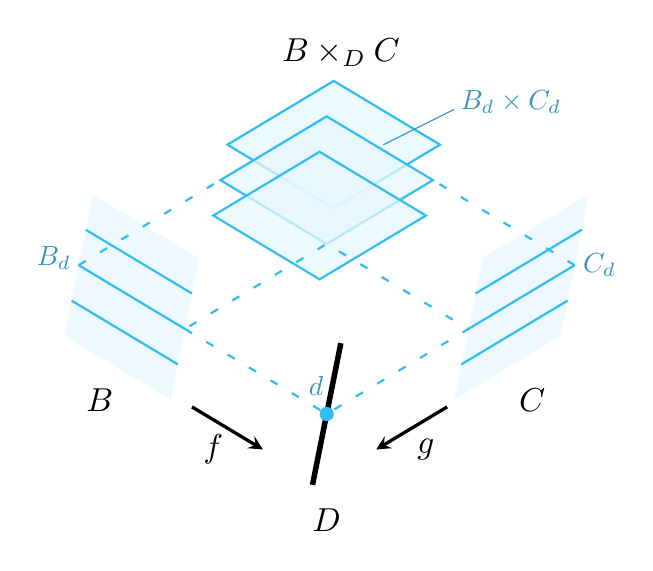
\begin{tikzpicture}[scale=.9]
        \draw [line width=2] (0, 0) -- (-.4, -2);
        \fill [cyan!7]
            (-2, 1.2) -- (-2.4, -.8) -- (-3.9, .1) -- (-3.5, 2.1);
        \fill [cyan!7]
            (2, 1.2) -- (1.6, -.8) -- (3.1, .1) -- (3.5, 2.1);
        \foreach \i in {1, ..., 3} {
            \draw [thick, cyan!80] 
                (-3.5 - .1 * \i, 2.1 - .5 * \i) -- (-2 - .1 * \i, 1.2 - .5 * \i)
                (3.5 - .1 * \i, 2.1 - .5 * \i) -- (2 - .1 * \i, 1.2 - .5 * \i);
        }
        \foreach \i in {1, ..., 3} {
            \draw [thick, cyan!80, fill=cyan!10, fill opacity=.75] 
                (-.1 * \i, 4.2 - .5 * \i) -- (1.5 - .1 * \i, 3.3 - .5 * \i) --
                (-.1 * \i, 2.4 - .5 * \i) -- (-1.5 - .1 * \i, 3.3 - .5 * \i) -- cycle;
        }
        \draw [thick, cyan!80, loosely dashed]
            (-2.2, .2) -- (-.2, -1) -- (1.8, .2) -- (-.2, 1.4) -- cycle
            (-3.7, 1.1) -- (-1.7, 2.3)
            (3.3, 1.1) -- (1.3, 2.3);
        \fill [cyan!80] (-.2, -1) circle (.1);
        \draw [line width=1.2, -stealth] (-2.1, -.9) -- (-1.1, -1.5);
        \draw [line width=1.2, -stealth] (1.5, -.9) -- (.5, -1.5);
        \node [cyan!75!black] at (-.35, -.6) {$d$};
        \node [scale=1.2] at (-.2, -2.5) {$D$};
        \node [scale=1.2] at (-3.4, -.8) {$B$};
        \node [scale=1.2] at (2.7, -.8) {$C$};
        \node [scale=1.2] at (-1.8, -1.5) {$f$};
        \node [scale=1.2] at (1.2, -1.5) {$g$};
        \node [scale=1.2] at (0, 4.1) {$B \times_D C$};
        \node [cyan!75!black] at (-4.05, 1.2) {$B_d$};
        \node [cyan!75!black] at (3.65, 1.1) {$C_d$};
        \node [cyan!75!black] at (2.4, 3.4) {$B_d \times C_d$};
        \draw [cyan!75!black] (1.6, 3.3) -- (.6, 2.8);
    \end{tikzpicture}\]
    $B \dtimes{D} C$ 被称为拉回, 也被称为是纤维积.
    \begin{definition} [拉回, 纤维积]
    \label{拉回}
    设 $\mathcal{C}$ 是 范畴 .
    对于 $\mathcal{C}$ 中的 交换图
    \[\begin{tikzcd}
	& B \\
	C & D
	\arrow["f"', from=1-2, to=2-2]
	\arrow["g", from=2-1, to=2-2]
    \end{tikzcd}\]
    如果这个图表具有 极限 ,
    就把这个极限叫做 $B, C$ 关于 $D$ 沿映射 $f, g$ 的\textbf{拉回}.

    具体地说, 该拉回是指交换图表
    \[\begin{tikzcd}
	{B \dtimes{D} C} & B \\
	C & D
	\arrow["{g'}", from=1-1, to=1-2]
	\arrow["{f'}"', from=1-1, to=2-1]
	\arrow["f"', from=1-2, to=2-2]
	\arrow["g", from=2-1, to=2-2]
    \end{tikzcd}\]
    它满足以下 万有性质 :
    对任意对象 $A' \in \mathcal{C}$, 如果有交换图表
    \[\begin{tikzcd}
	{A'} & B \\
	C & D
	\arrow["{g''}", from=1-1, to=1-2]
	\arrow["{f''}"', from=1-1, to=2-1]
	\arrow["f"', from=1-2, to=2-2]
	\arrow["g", from=2-1, to=2-2]
    \end{tikzcd}\]
    则存在唯一的态射 $h \colon A' \to A$, 使得以下图表交换:
    \[\begin{tikzcd}
	{A'} \\
	& {B \dtimes{D} C} & B \\
	& C & D
	\arrow["{\exists! h}"{description}, dashed, from=1-1, to=2-2]
	\arrow["{g''}", curve={height=-18pt}, from=1-1, to=2-3]
	\arrow["{f''}"', curve={height=18pt}, from=1-1, to=3-2]
	\arrow["{g'}"', from=2-2, to=2-3]
	\arrow["{f'}", from=2-2, to=3-2]
	\arrow["f"', from=2-3, to=3-3]
	\arrow["g", from=3-2, to=3-3]
    \end{tikzcd}\]
    \end{definition}
    而其对偶构造被称为推出, 也称为纤维余积, 比如说对于图表 
    \[\begin{tikzcd}
	& B \\
	C & D
	\arrow["f"', from=2-2, to=1-2]
	\arrow["g", from=2-2, to=2-1]
    \end{tikzcd}\]
    的推出记为 $B \dsqcup{D} C$.
\end{example}
\begin{exercise}
    请读者使用我们刚刚的思路思考拉回和推出分别代表什么, 此外, 说明拉回相当于``原像'', 推出相当于``像''.
\end{exercise}
接下来我们讲述极限的第二种刻画方式: 令 $I^{\triangleleft}$ 和 $I^{\triangleright}$ 为在 $I$ 中形式地添加一个始对象或终对象, 即将图表变为
\[\begin{tikzcd}
	& \varnothing \\
	i && j
	\arrow[from=1-2, to=2-1]
	\arrow[from=1-2, to=2-3]
	\arrow[from=2-1, to=2-3]
\end{tikzcd} \quad\text{和} \quad \begin{tikzcd}
	i && j \\
	& {*}
	\arrow[from=1-1, to=1-3]
	\arrow[from=1-1, to=2-2]
	\arrow[from=1-3, to=2-2]
\end{tikzcd}\]
此时有显然的函子 $I\to I^{\triangleleft}$ 和 $I \to I^{\triangleright}$. 此时考虑拉回(相当于限制态射对于 $\alpha$ 一点取逆)
\[\begin{tikzcd}
	{\Fct_\alpha{(I^{\triangleleft},\cal{C})}} & {\Fct(I^{\triangleleft},\cal{C})} \\
	{*} & {\Fct(I,\cal{C})}
	\arrow[from=1-1, to=1-2]
	\arrow[from=1-1, to=2-1]
	\arrow["{\text{限制}}"', from=1-2, to=2-2]
	\arrow["\alpha", from=2-1, to=2-2]
\end{tikzcd}\]
我们就得到 $\Fct_{\alpha}(I^{\triangleleft},\cal{C})$ 称其为锥, 此时其中对象可以表为(不难发现限制在 $I$ 上为 $\alpha$).
\[\begin{tikzcd}
	& X \\
	{\alpha(i)} && {\alpha(j)}
	\arrow[from=1-2, to=2-1]
	\arrow[from=1-2, to=2-3]
	\arrow["{\alpha(i\to j)}", from=2-1, to=2-3]
\end{tikzcd}\]
因此考虑其中终对象即为极限. 反过来, 考虑 $\Fct_{\alpha}(I^{\triangleright},\cal{C})$ 其始对象就是余极限.\\
现在, 我们在集合范畴 $\cate{Set}$ 中刻画极限, 这一过程相当于在求解规划问题\footnote{当然, 这样可能并不严谨.}
\begin{align*}
    \min & \quad \prolim \alpha \in \cal{C}\\
    \op{s.t.} &\left\{
    \begin{array}{ccc}
         \prolim \alpha \to \alpha(i),& \forall i\in \Obj(I) \\
         \alpha(i) \xrightarrow{\alpha(i\to j)} \alpha(j), & \forall (i\to j) \in \Mor(I)\\
         \text{上述全体箭头均交换}
    \end{array}
    \right.
\end{align*}
我们可以分成两步来求解该规划问题, 首先解决 $\prolim \alpha \to \alpha(i)$, 这无非是在说将 $I$ 先视为离散范畴进行求解, 直接得到结果为积 $\prod_{I} \alpha(i)$. 而后不断加入条件, 不难发现, 在集合范畴中, 增加这些条件相当于得到以下集合
\[
\left\{(x_i)_{i\in \Obj(I)} \colon \forall (i\xrightarrow{\sigma} j) \in\Hom(i,j), \alpha(\sigma)(x_i) = x_j\right\}.
\]
而该操作对于一般具体的范畴也是使用的, 这估计就是古老文献中, 将极限称为``普适问题的解''的原因所在.\\
现在我们来刻画余极限, 这与极限是对偶的.
\begin{align*}
    \max & \quad \indlim \alpha \in \cal{C}\\
    \op{s.t.} &\left\{
    \begin{array}{ccc}
           \alpha(i)\to \indlim \alpha,& \forall i\in \Obj(I) \\
         \alpha(i) \xrightarrow{\alpha(i\to j)} \alpha(j), & \forall (i\to j) \in \Mor(I)\\
         \text{上述全体箭头均交换}
    \end{array}
    \right.
\end{align*}
由于此时为 $\alpha(i) \to \indlim \alpha$, 因此我们可以先考虑 $\alpha(i) \xrightarrow{\alpha(i\to j)}\alpha(j)$, 这相当于说在生成元上具有一些关系 : 对于 $x_i \in \alpha(i)$, 有 $x_i \sim x_j \Leftrightarrow \alpha(i\to j)(x_i) = x_j$. \\
然后我们来考虑由此生成的 $\indlim \alpha$, 这无非是在说先使用 $\alpha(i)$ 自由生成 $\indlim \alpha$, 而后商去这些关系(读者可以想象为某种群展示, 当然群展示确实也是一种余极限), 得到:
\[
    \coprod_{i\in I} \alpha(i) /\sim
\]
一般而言, 我们喜欢在滤过的东西上讨论余极限, 首先容许我介绍一下何谓滤过:

\subsection{应用 : Kan 延拓}
\subsection{伴随函子}
\subsection{可表函子}
\subsection{幺半范畴}

\section{方便的空间范畴}
本节来讲述方便的空间范畴概念, 一般来说, 方便的空间范畴指的是拓扑空间范畴中满足以下条件的饱和\footnote{replete, 子范畴 $\cal{D}$ 称为是饱和的, 指对于任意 $x\in \cal{D}$, 若在 $\cal{C}$ 中有 $f \colon y \simeq x$, 则 $f$ 和 $y$ 都在 $\cal{D}$ 中.}全子范畴. 本节主要参考\cite{StricklandCGWH}以及\cite[7.好用的空间范畴]{李思}
\begin{definition}[方便的空间范畴]
    称 $\cal{C}$ 为\textbf{方便的空间范畴}, 指其为 $\cate{Top}$ 的饱和全子范畴, 并且满足以下三条条件
    \begin{itemize}
        \item 每个 CW 复形均为 $\cal{C}$ 中的对象.
        \item $\cal{C}$ 是 Cartesian 闭的(定义~\ref{定义:Cartesian闭}, 或者说具有指数律).
        \item $\cal{C}$ 是完备且余完备的.
    \end{itemize}
\end{definition}
首先介绍闭幺半范畴的概念
\begin{definition}[闭幺半范畴]
    设$\mathcal{C}$为幺半范畴.当以下条件成立时,称$\mathcal{C}$为右(或左)闭幺半范畴:对所有对象$Y$,函子$ - \otimes Y : \mathcal{C} \to \mathcal{C}$(或$Y\otimes - : \mathcal{C} \to \mathcal{C}$)带有指定的右伴随.兼具左闭和右闭的幺半范畴称为闭幺半范畴.
\end{definition}
\begin{remark}
    我们考虑的幺半范畴均为辫幺半范畴,因此无需区分左闭右闭,此时$- \otimes Y$的右伴随记为$\underline{\Hom}(Y,-)$.
\end{remark}
一般而言,对任意范畴$\mathcal{C}_1$和$\mathcal{C}_2$之间的两对伴随函子$(F,G)$和$(F',G')$,任何$\varphi :F \to F'$都自然诱导了$\psi : G' \to G$.相反也是如此.诱导态射由交换图表
\[\begin{tikzcd}
	{\Hom(F'X,Y)} & {\Hom(X,G'Y)} \\
	{\Hom(FX,Y)} & {\Hom(X,GY)}
	\arrow["\sim"', from=1-1, to=1-2]
	\arrow["{(\varphi_X)^*}", from=1-1, to=2-1]
	\arrow["{(\psi_Y)_*}"', from=1-2, to=2-2]
	\arrow["\sim", from=2-1, to=2-2]
\end{tikzcd}\]
刻画.\\

作为应用,闭幺半范畴中的任何态射$Y \to Y'$诱导$\underline{\Hom}(Y', -)\to \underline{\Hom}(Y, -)$,所以闭幺半范畴的性质相当于在说存在双函子$\underline{\Hom}(-,-):\mathcal{C}^{\opposite} \times \mathcal{C} \to \mathcal{C}$以及一族典范双射
\begin{equation}\label{公式:内 Hom}
\tag{内 Hom}
   \Hom(X\otimes Y,Z) \simeq \Hom\left(X,\underline{\Hom}(Y,Z)\right), 
\end{equation}

它对于三个变元皆有函子性.\\

双函子$\underline{\Hom}(-,-)$也称为闭幺半范畴$\mathcal{C}$的内Hom.定义导致以下结论:
\begin{itemize}
    \item $\Hom(X,Z) \simeq \Hom(X\otimes \one,Z) \simeq \Hom(X,\underline{\Hom}(\one,Z))$,再由米田引理可知$Z \simeq \underline{\Hom}(\one,Z)$.
    \item 伴随对的单位态射给出$\coev_{X,Y}:X\to  \underline{\Hom}(Y,X\otimes Y)$,余单位态射给出$\ev_{Y,X}:\underline{\Hom}(Y,X)\otimes Y \to X$.
    \item 从合成
    \[\underline{\Hom}(Y,Z)\otimes(\underline{\Hom}(X,Y)\otimes X) \xrightarrow{\identity\otimes\ev_{X,Y}}\underline{\Hom}(Y,Z)\otimes Y\xrightarrow{\ev_{Y,Z}}Z\]
    以及伴随性质和结合约束可得
    \[
    \underline{\Hom}(Y,Z)\otimes\underline{\Hom}(X,Y)\to \underline{\Hom}(X,Z).
    \]
    \item 取$\coev_{\one,X}$得$\one \to \underline{\Hom}(X,X)$.
\end{itemize}
不难得到
\begin{proposition}
    设$\mathcal{C}$是闭幺半范畴,则有一族典范双射
    \[
    \Hom(X,Y) \simeq \Hom(\one,\underline{\Hom}(X,Y)),\quad X,Y \in \Obj(\mathcal{C}).
    \]
\end{proposition}
这说明内Hom可以得到Hom.\\

此外,伴随也可以内化到$\mathcal{C}$.
\begin{proposition}
    设$\mathcal{C}$是闭幺半范畴,则有一族同构
    \[
    \underline{\Hom}(X\otimes Y,Z)\simeq \underline{\Hom}(X,\underline{\Hom}(Y,Z));
    \]
    更精确地说,这是从$\mathcal{C}^{\opposite}\times \mathcal{C}^{\opposite}\times \mathcal{C} \to \mathcal{C}$的函子间的同构.
\end{proposition}
\begin{proof}
    考虑$\Hom(T,\underline{\Hom}(X\otimes Y,Z))$利用结合约束以及伴随同构证明
    \[\Hom(T,\underline{\Hom}(X\otimes Y,Z))\rightiso \Hom(T,\underline{\Hom}(X,\underline{\Hom}(Y,Z)))
    \]
    结合Yoneda引理可知结果.
\end{proof}
引入闭幺半范畴是为了进一步约化到双函子$\otimes$为积$\times$的情况,在这一情况下,会增加一个有趣的观察.
\begin{definition}[Cartesius闭]\label{定义:Cartesian闭}
    设$\mathcal{C}$是具备有限积的范畴.如果$(\mathcal{C},\times)$为闭幺半范畴,则称$\mathcal{C}$为Cartesius闭的. 此时内 Hom 称为\textbf{指数对象}, 在拓扑中, 我们称其满足指数律.
\end{definition}
\begin{example}
\begin{enumerate}
    \item 集合范畴$\cate{Set}$是Cartesius闭的:取$\underline{\Hom}(X,Y) = Y^X$即可.
    \item 取$\mathcal{C} = \cate{Top}$,它具有许多良好性质,并且对积$\times$构成对称幺半范畴,但是它不是 Cartesian 闭的.
    \item 考虑全体小范畴构成的范畴$\cate{Cat}$,其中积为$\cal{C}_1\times \cdots \cal{C}_n$,而空积为$\bold{1}$.范畴$\cate{Cat}$是 Cartesian 闭的,这来自于以下简单的论断:指定双函子$\cal{A} \times \cal{B} \to \cal{C}$相当于指定函子$\cal{A} \to \cal{C}^{\cal{B}}$也相当于指定函子$\cal{B} \to \cal{C}^{\cal{A}}$.
\end{enumerate}
\end{example}
由于映射空间在拓扑学中俯拾即是,为解决$\cate{Top}$不是 Cartesian 闭的问题,我们引入紧生成空间与紧生成弱 Hausdorff 空间.两者都是方便的空间范畴,在$\infty$-范畴理论中,使用紧生成弱 Hausdorff 空间更多一些.\\
首先,回顾一下紧生成空间的定义,根据Bourbaki的定义,紧空间意谓紧且Hausdorff的空间.
\begin{definition}[弱Hausdorff]\label{定义:弱Hausdorff}
    设$X$为拓扑空间, $K$为紧空间,若对于任意连续映射$f: K \to X$都有$f(K)$是$X$中的闭集,则称$X$是弱Hausdorff的.
\end{definition}
\begin{example}
    Hausdorff空间是弱 Hausdorff 的.
\end{example}
这种空间的分离性介于T$_1$与Hausdorff之间.
\begin{definition}[紧闭子空间]\label{定义:紧闭子空间}
    设$X$为拓扑空间, $A \subset X$为其子空间, $K$为紧空间,若对于任意映射$f : K \to X$都有$f^{-1}(A)$为$K$中的闭集,则称$A$是$X$的紧闭子空间.\footnote{注意,不一定在$X$上闭}
\end{definition}
\begin{definition}[Kelly空间]
    设$X$为拓扑空间,若其每个紧闭子空间在$X$上都是闭的,则称$X$为Kelly空间,简称$k$-空间.
\end{definition}
\begin{definition}[紧生成空间]\label{定义:紧生成空间}
    设$X$为拓扑空间,以$X$中的紧闭子集作为闭集构成一个新的拓扑空间$kX$,有恒等映射$kX \to X$.若$kX = X$,则称$X$是紧生成的.记$\cate{CG}$为$\cate{Top}$中所有紧生成空间构成的范畴,当然也可以说是$k$-空间构成的范畴.
\end{definition}
\begin{proposition}\label{命题:紧生成化与嵌入函子伴随}
    由$X \mapsto kX$给出的函子$k : \cate{Top} \to \cate{CG}$是嵌入函子$\iota: \cate{CG} \to \cate{Top}$的右伴随.
\end{proposition}
\begin{proof}
    记$X \in \cate{CG}$, $Y\in \cate{Top}$,欲证
    \[
    \Hom_{\cate{CG}}(X,kY)\simeq \Hom_{\cate{Top}}(\iota X,Y),
    \]
    只需证明$f : X \to Y$连续当且仅当$f : X \to kY$连续即可.
    \begin{enumerate}
        \item[($\Rightarrow$)]假设$f: X\to Y$连续,则令$Z \subset Y$为紧闭子集考虑$f^{-1}(Z)$.对任意紧空间$K$,映射$g: K \to X$,由于$f\circ g : K \to Y$,因此$(f\circ g)^{-1}(Z)$在$K$中是闭的,这意味着$f^{-1}(Z)$为$X$中的紧闭子集,而$X$为紧生成空间,即$f^{-1}(Z)$在$X$中闭,从而$kY$中的闭集在$f$的逆像为$X$中的闭集从而$f: X \to kY$连续.
        \item[($\Leftarrow$)]由于$kY \to Y$连续,因此考虑复合即可.
    \end{enumerate}
\end{proof}
\begin{proposition}\label{Pro:紧生成空间商映射}
    若$X \in \cate{CG}$, $\pr: X\to Y$为商映射,则$Y\in \cate{CG}$.
\end{proposition}
\begin{proof}
    由于商映射为使得$\pr : X \to Y$连续的最细的映射且有分解$\pr : X \to kY \to Y$,因此$Y = kY$.
\end{proof}
\begin{theorem}[$\cate{CG}$的完备性]
    范畴$\cate{CG}$完备且余完备.其余极限继承相应空间在$\cate{Top}$中的余极限,而极限由$k$作用于相应空间在$\cate{Top}$中的极限得到.
\end{theorem}
\begin{proof}
    设$\mathcal{I}$为指标范畴, $F \in \Fct(\mathcal{I},\cate{CG})$, $\hat{F} = \iota \circ F$.由于$\iota$为左伴随,保$\indlim$,因此只需要证明$\cate{CG}$中对象在$\cate{Top}$的余极限仍在$\cate{CG}$中即可,由于命题\ref{Pro:紧生成空间商映射},只需要证明$\bigsqcup_{i\in \mathcal{I}}F(i)$在$\cate{CG}$中即可,这是显然的.而后由于$k$为右伴随,因此保$\prolim$,即
    \[
    \underset{i\in \mathcal{I}}{\prolim} F(i) = \underset{i\in \mathcal{I}}{\prolim} (k\circ \hat{F}(i)) = k \underset{i\in \mathcal{I}}{\prolim} \hat{F}(i).
    \]
\end{proof}
\begin{corollary}
    令$\{X_i\}_{i\in I}$为$\cate{CG}$中的一族对象.则它们在$\cate{CG}$中的乘积为
    \[
     k(\prod_{i\in I}X_i)
    \]
    此处$\prod_{i\in I}X_i$为在拓扑空间中的乘积.
\end{corollary}
\begin{definition}[紧生成弱Hausdorff空间]\label{Def:紧生成弱Hausdorff空间}
    设$X$为拓扑空间,若其是弱Hausdorff的$k$-空间,则称其为紧生成空间,其构成的范畴记为$\cate{CGWH}$.
\end{definition}
\begin{proposition}
    设$X$为弱Hausdorff空间, $K$为紧空间,若$f : K \to X$连续,则$f(K)$为紧空间.
\end{proposition}
\begin{proof}
    由于$K$紧且$X$弱Hausdorff,由定义即知$f(K)$闭,而由连续映射保持紧性知$f(K)$紧,此外得知$f$为闭映射.而后考虑$x_1,x_2 \in f(K)$由于$X$为弱Hausdorff空间, $\{x_1\}$和$\{x_2\}$为闭子集,因此考虑其逆像得知$f^{-1}(x_1)$与$f^{-1}(x_2)$无交,而$K$紧Hausdorff,从而存在$U_1,U_2$为$K$中开集使得$f^{-1}(x_1)\in U_1$而$f^{-1}(x_2)\in U_2$,即$x_2\in K-U_1$而$x_1 \in K-U_2$.考虑$f(K) - f(K-U_i)$($i=1,2$)便得到包含$x_1$和$x_2$的无交开集.
\end{proof}
\begin{proposition}
    设$X$为紧生成空间,则$X$弱Hausdorff当且仅当对角线子空间$\delta_X$在$X\times X$中闭,此处$X \times X$为$\cate{CG}$中的乘积.
\end{proposition}
\begin{proof}
    设$X \in  \cate{CGWH}$,现证$\delta_X$紧闭.考虑
    \[
    f=(f_1,f_2) : K \to X\times X, f_i : K \to X
    \]
    $K$为紧空间,记
    \[
    L = f_1(K) \cap f_2(K)
    \]
    可知$L$为紧空间.考虑对角线$\delta_L$,由于$L$为紧空间, $\delta_L$为$X\times X$的紧子空间,而$X$紧生成,因此$\delta_L$在$X\times X$中闭.即$f^{-1}(\delta_X) = f^{-1}(\delta_L)$闭.\\
    反过来只需证明若$K$为紧空间$f: K\to X$连续,则$f(K)$紧闭即可.不妨设$L$为紧空间, $g: L \to X$连续,考虑
    \[
    (f,g): K \times L \to X\times X.
    \]
    则
    \[
    g^{-1}(f(K)) = (f,g)^{-1}(\delta_X)
    \]
    为闭集,即$f(K)$紧闭.
\end{proof}
\begin{corollary}\label{Cor:CG乘积也在CGWH中}
    设$\{X_i\}$为$\cate{CGWH}$中的一族对象,则它们在$\cate{CG}$的乘积也在$\cate{CGWH}$中.
\end{corollary}
\begin{proposition}
    函子$h : \cate{CG} \to \cate{CGWH}$是嵌入$\iota': \cate{CGWH}\to \cate{CG}$的左伴随.
\end{proposition}
\begin{theorem}[$\cate{CGWH}$的完备性]\label{The:CGWH的完备性}
    范畴$\cate{CGWH}$完备且余完备.极限继承自$\cate{CG}$而余极限来自$h$作用于$\cate{CG}$.
\end{theorem}
\begin{proof}
    与$\cate{CG}$完备且余完备的证明是类似的.唯一不平凡的是需要使用推论\ref{Cor:CG乘积也在CGWH中}即可得知乘积存在,而后由范畴中构造极限的方式可以证明极限确实继承自$\cate{CG}$.
\end{proof}
\begin{proposition}
    $\cate{CGWH}$是 Cartesian 闭的.
\end{proposition}
\begin{proof}   
见\parencite[Proposition 2.12]{StricklandCGWH}
\end{proof}